\subsection{Echo chambers}
Dealing with news media, \textit{echo chamber} is a metaphorical description
of a situation in which beliefs are amplified or reinforced by
communication and repetition inside a closed
system.\cite{echochamwiki,echocham}\\
With respect to quality, we studied the presence of echo chambers
in our network.
First of all, our agents have a ``mental  state'', i.e. a vector of
preferences: its components represent the amount of interests toward
a certain topic.\\
News have the same dimension of \textit{mental state vector} (MSV)
in order to establish a ``matching'' between news' topics and users'
preferences.
MSV is highly involved in news' dynamics and network
topology.\footnote{See section~\nameref{introduction} for more
  details on the previous work.}\\
In the images below we extracted main clusters from our network using
MSV size of three, five and seven.
Memory length was set to twelve for all the simulations.\\
\textit{Modularity} is a measure for detecting community
structure in graphs.\cite{modulwiki}
To exhibit a comparison between the tree runs,
nodes were painted with colors representing modularity class
(figures~\ref{fig:bubble3mod},~\ref{fig:bubble5mod} and~\ref{fig:bubble7mod})
and the most recent news in memory
(figures~\ref{fig:bubble3news},~\ref{fig:bubble5news} and~\ref{fig:bubble7news}).
When news are homogeneous inside a single cluster, we observe
an echo chamber.\\
We point out that the number of clusters is the MSV size.
Concerning news, the state is more heterogeneous:
although some clusters still exist, there is not a clear separation
among users with different news.
%
\begin{figure}
  \centering
  \begin{subfigure}[t]{0.25\textwidth}
    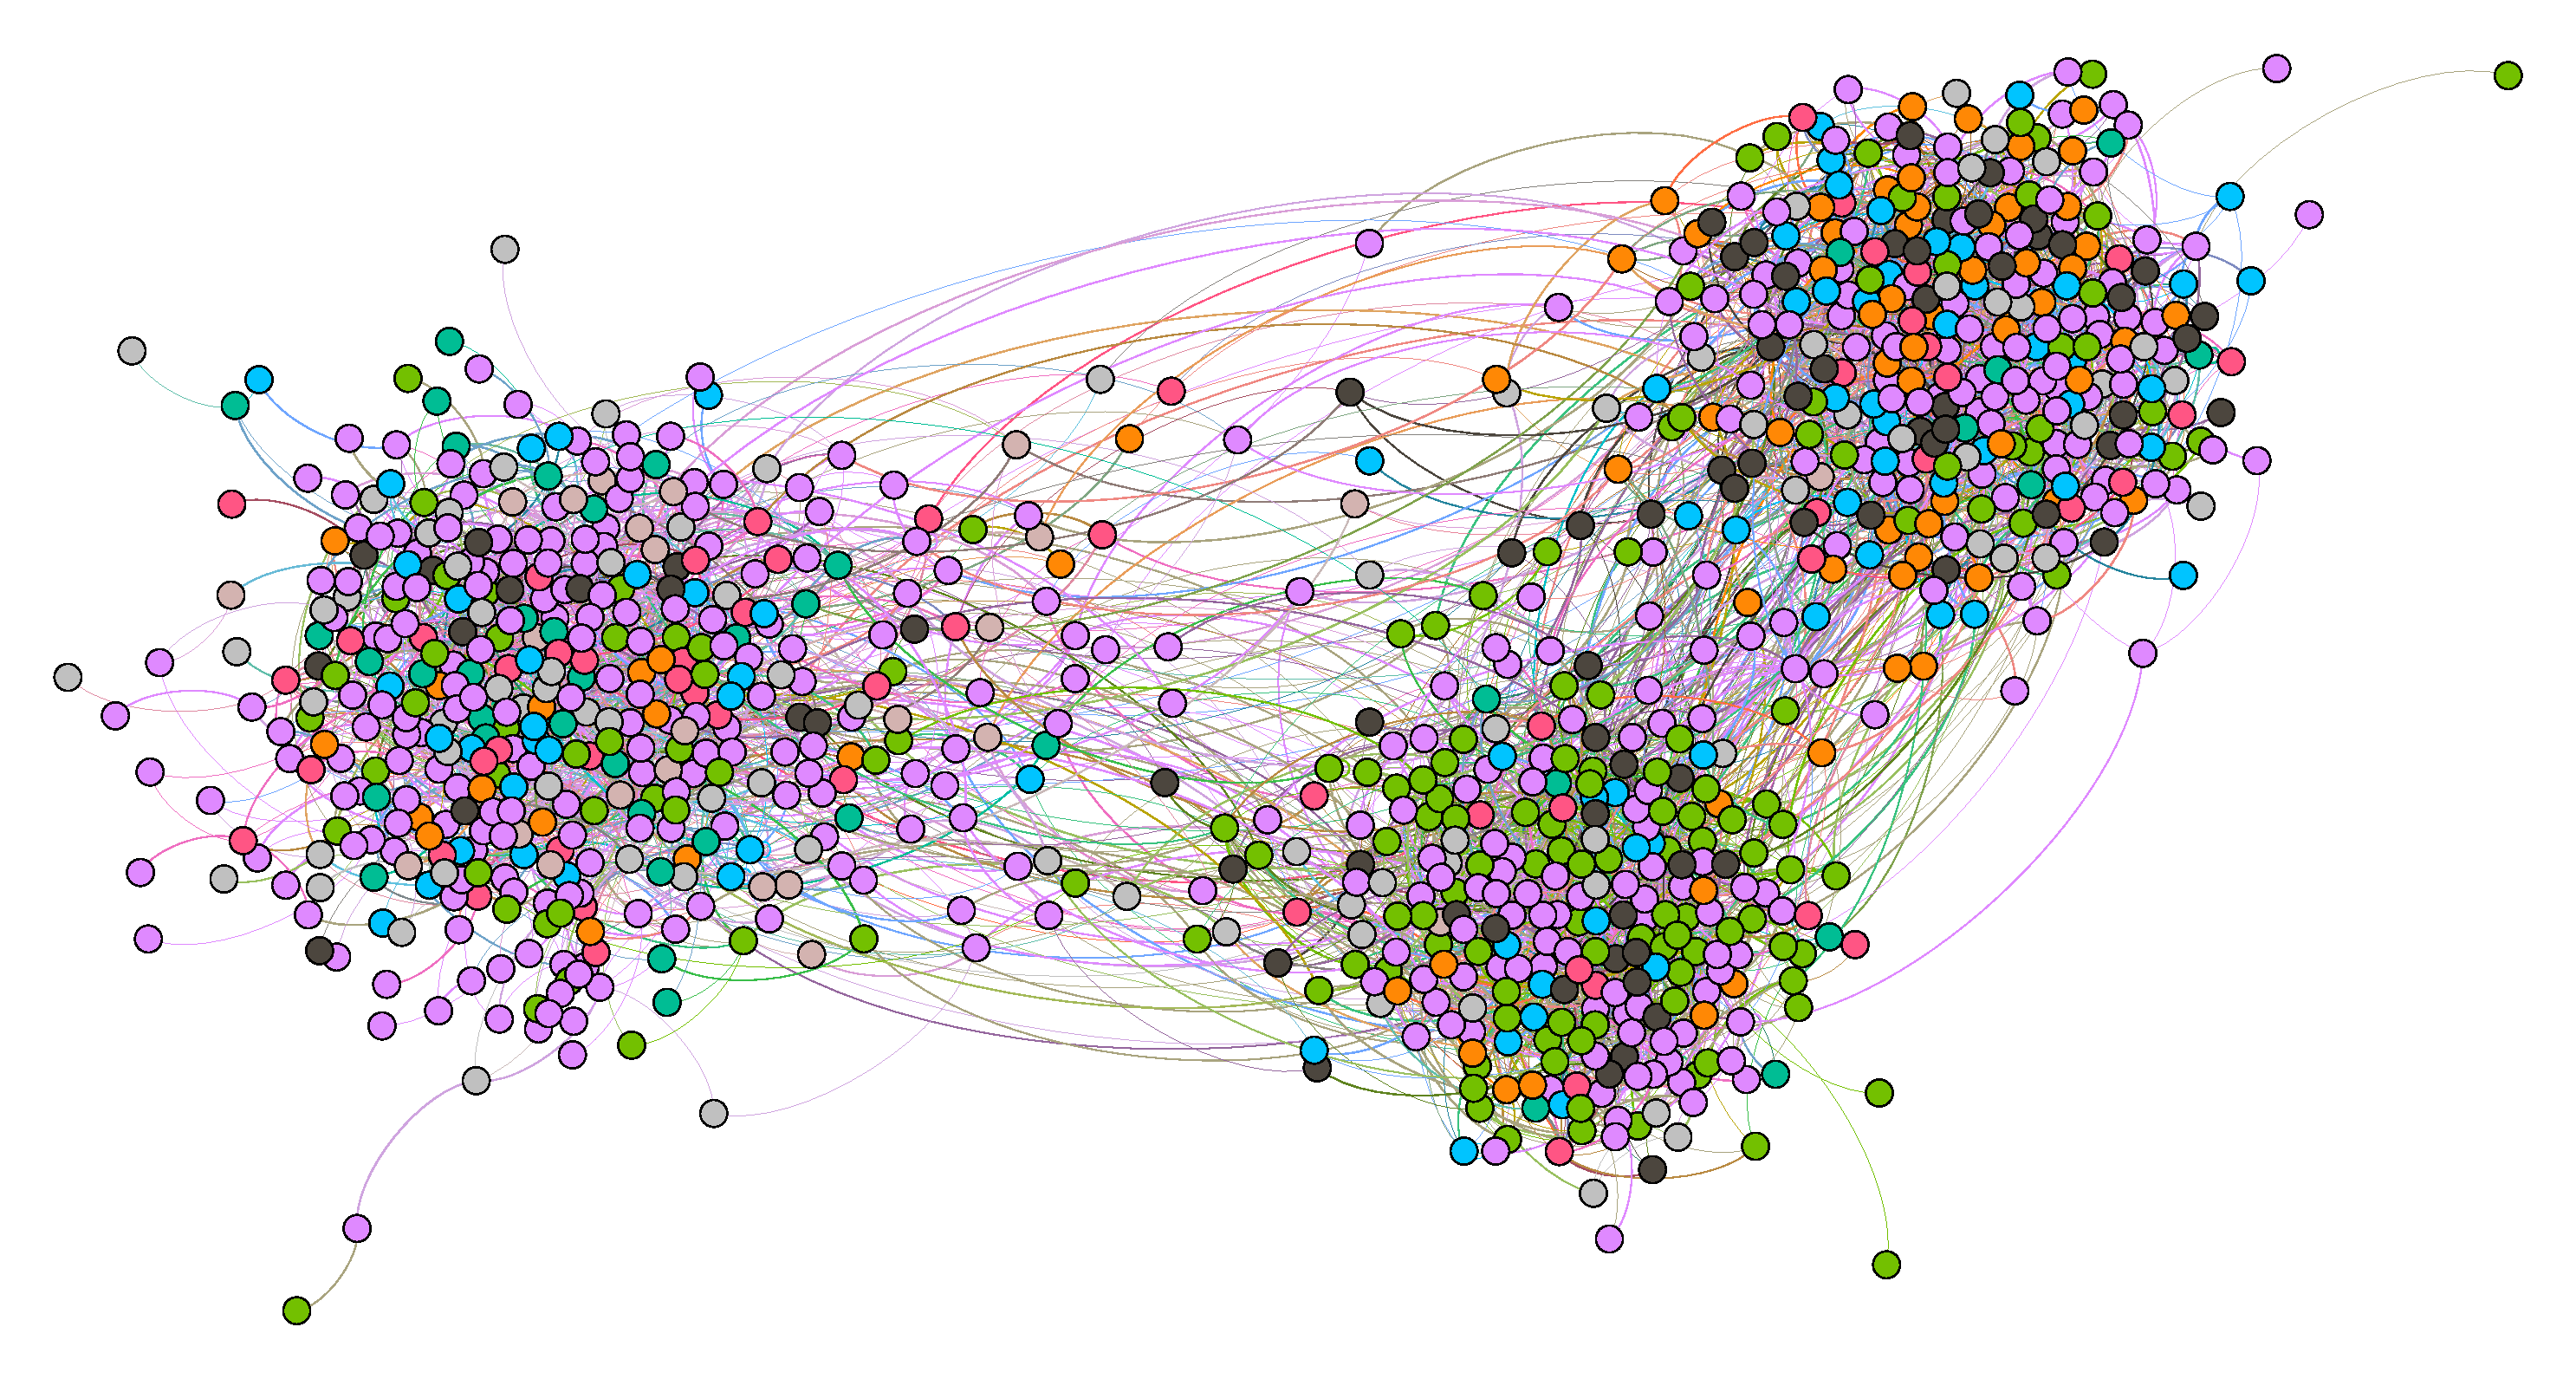
\includegraphics[width=\textwidth]{img/dim3_mod.pdf}
    \caption{State vector dimension: 3.
      Modularity class highlighted.}
    \label{fig:bubble3mod}
  \end{subfigure}
  ~
  \begin{subfigure}[t]{0.35\textwidth}
    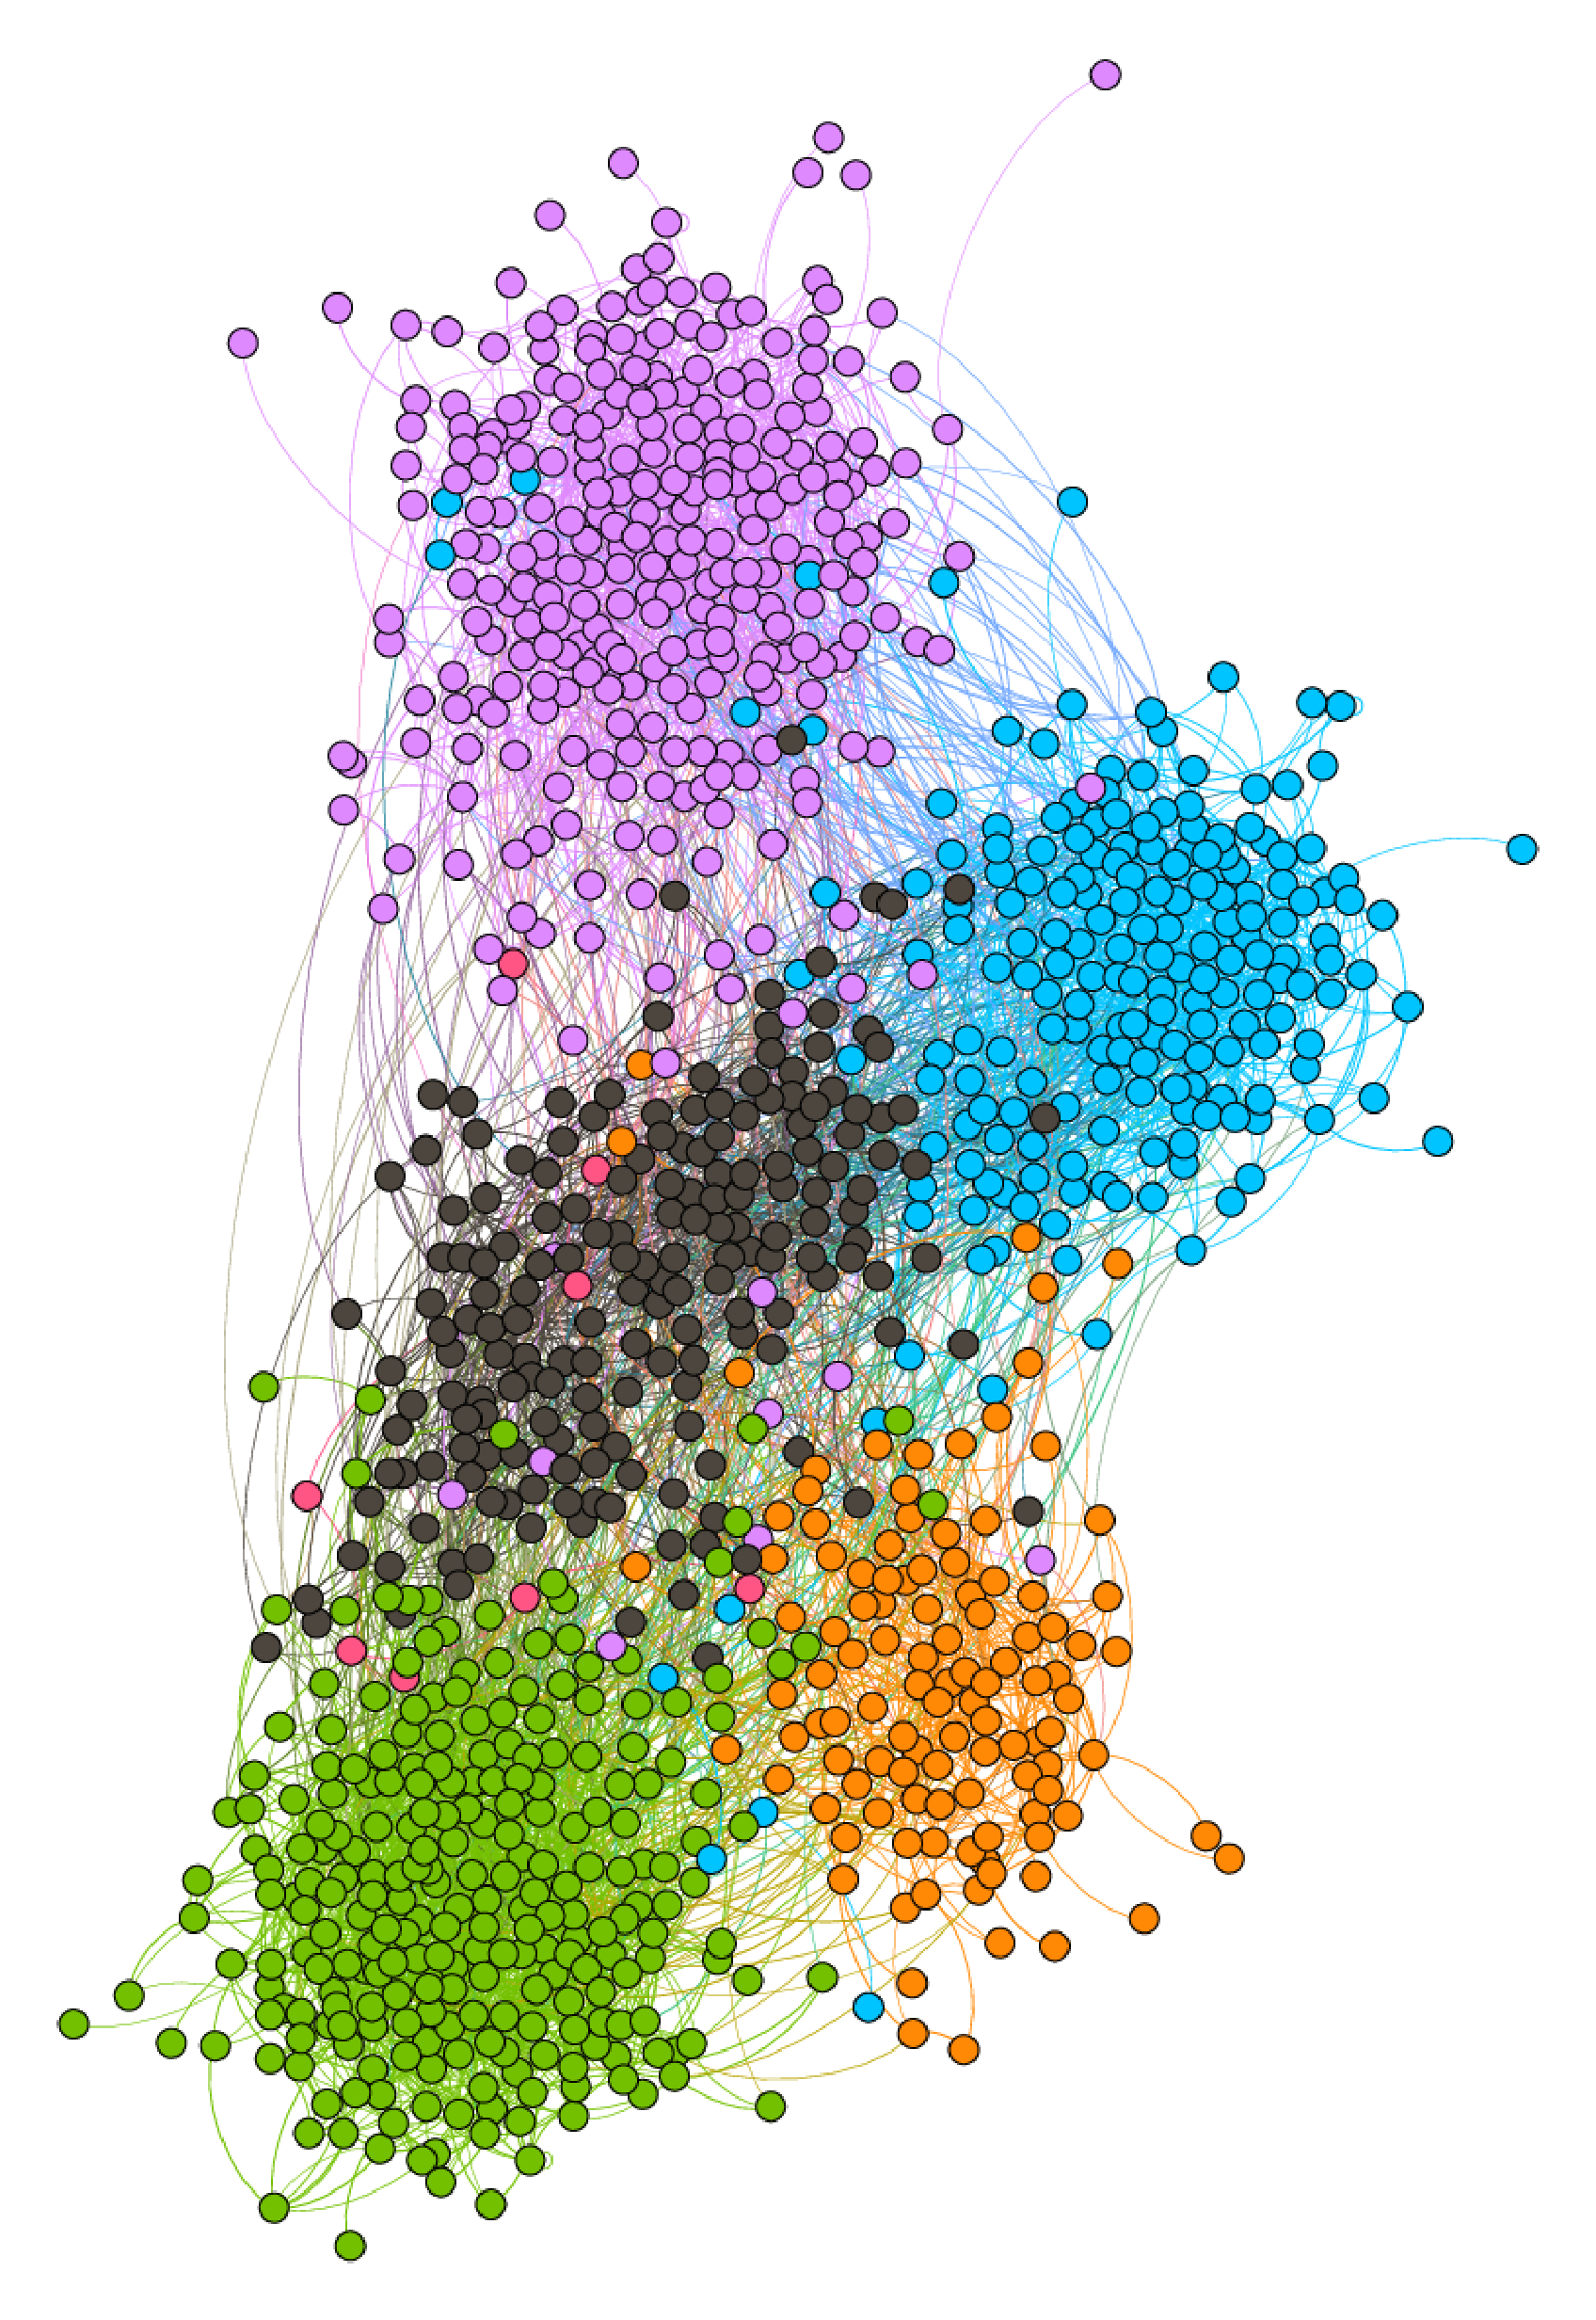
\includegraphics[width=\textwidth]{img/dim5_mod.pdf}
    \caption{State vector dimension: 5.
      Modularity class highlighted.}
    \label{fig:bubble5mod}
  \end{subfigure}
  ~
  \begin{subfigure}[t]{0.35\textwidth}
    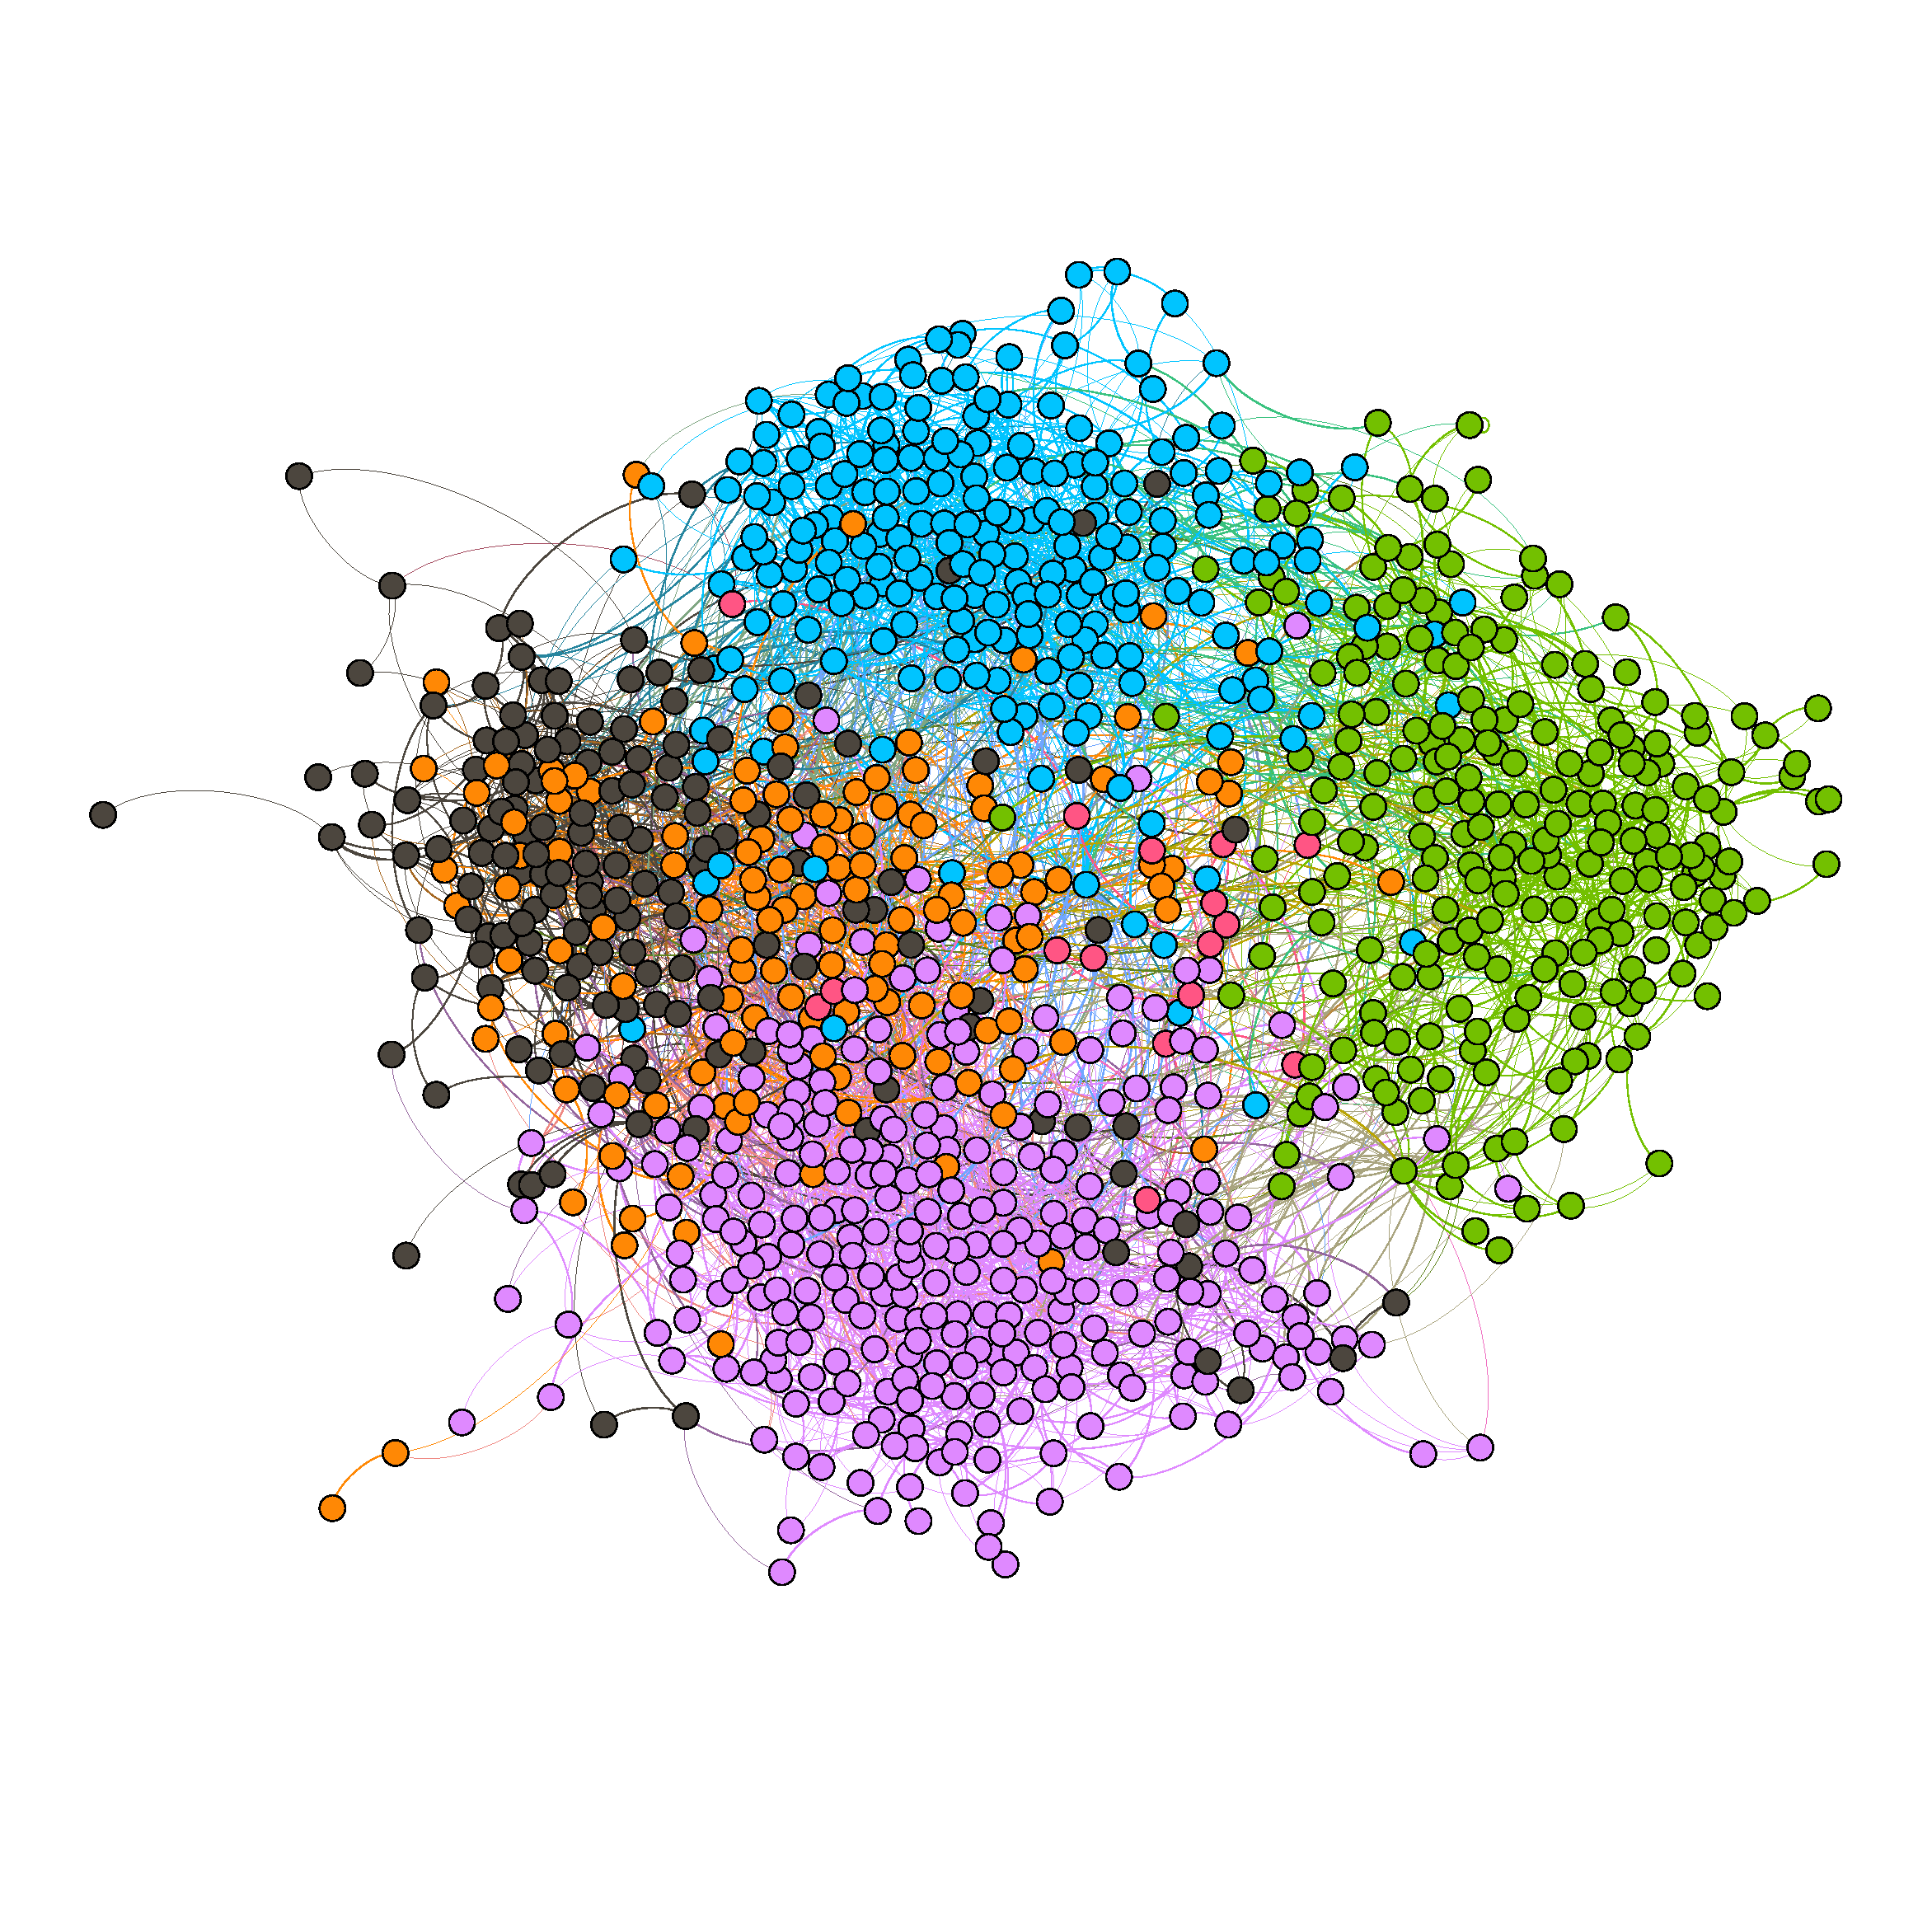
\includegraphics[width=\textwidth]{img/dim7_mod.pdf}
    \caption{State vector dimension: 7.
      Modularity class highlighted.}
    \label{fig:bubble7mod}
  \end{subfigure}
  \\
  \begin{subfigure}[t]{0.25\textwidth}
    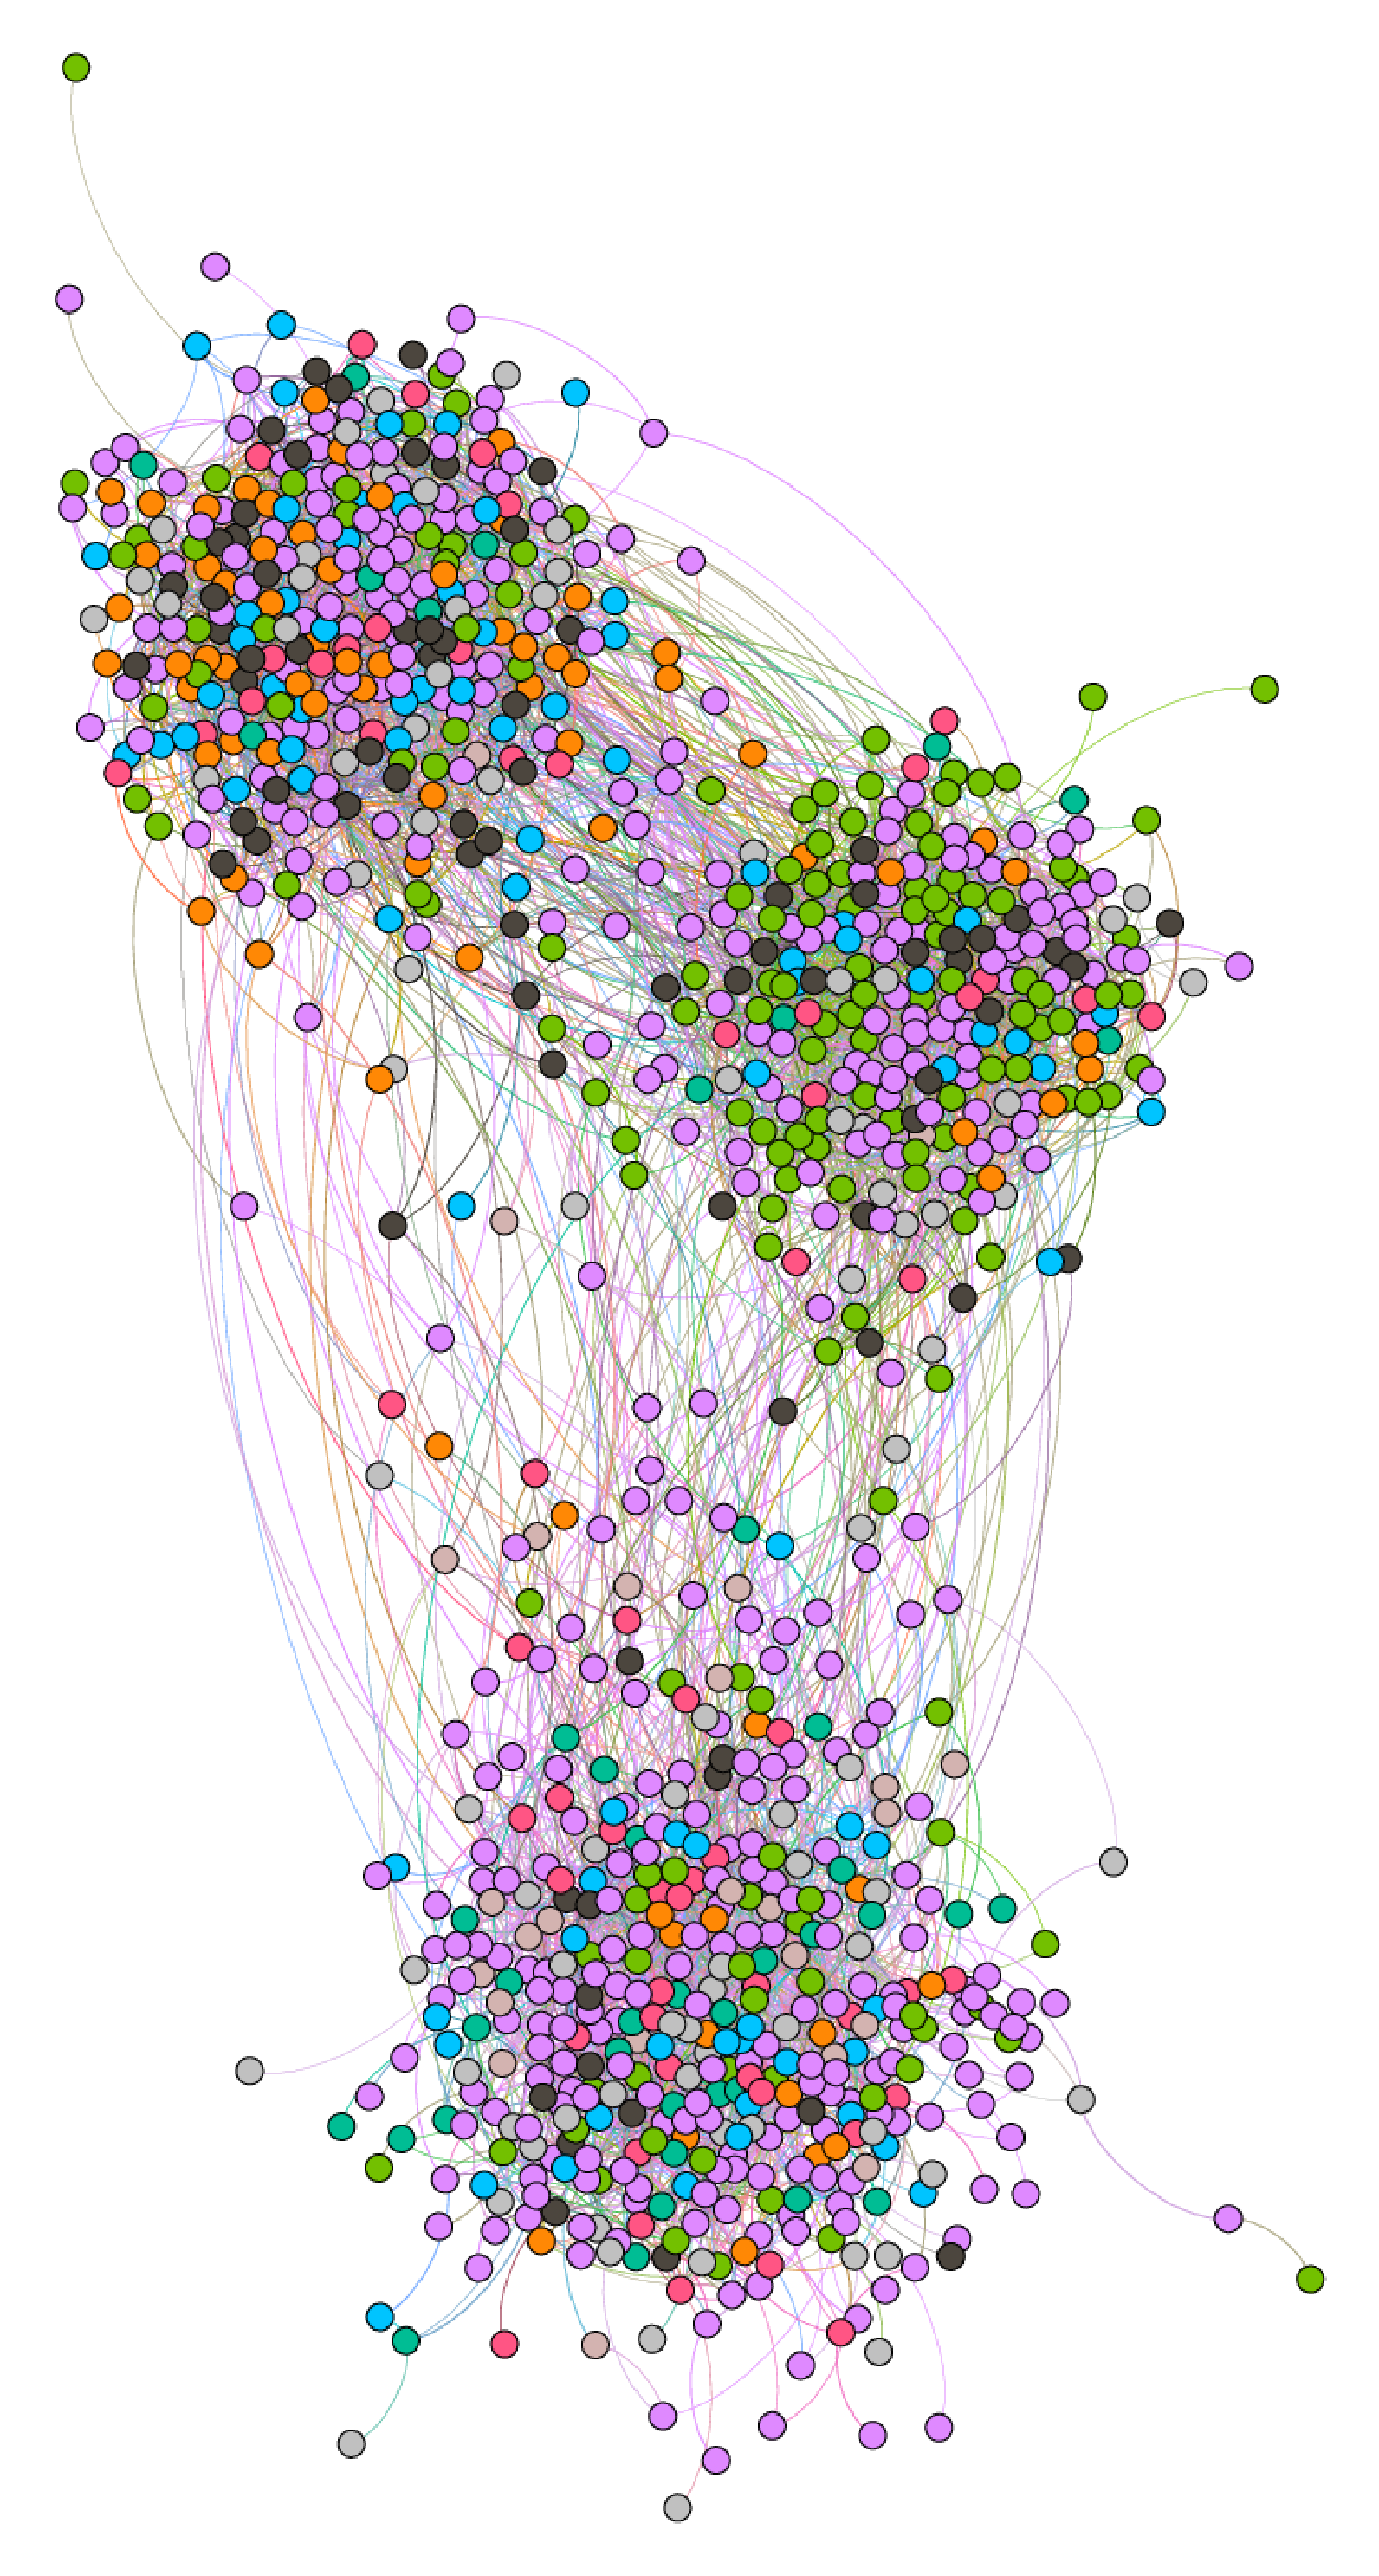
\includegraphics[width=\textwidth]{img/dim3_news.pdf}
    \caption{State vector dimension: 3.
      Latest news highlighted.}
    \label{fig:bubble3news}
  \end{subfigure}
  ~
  \begin{subfigure}[t]{0.35\textwidth}
    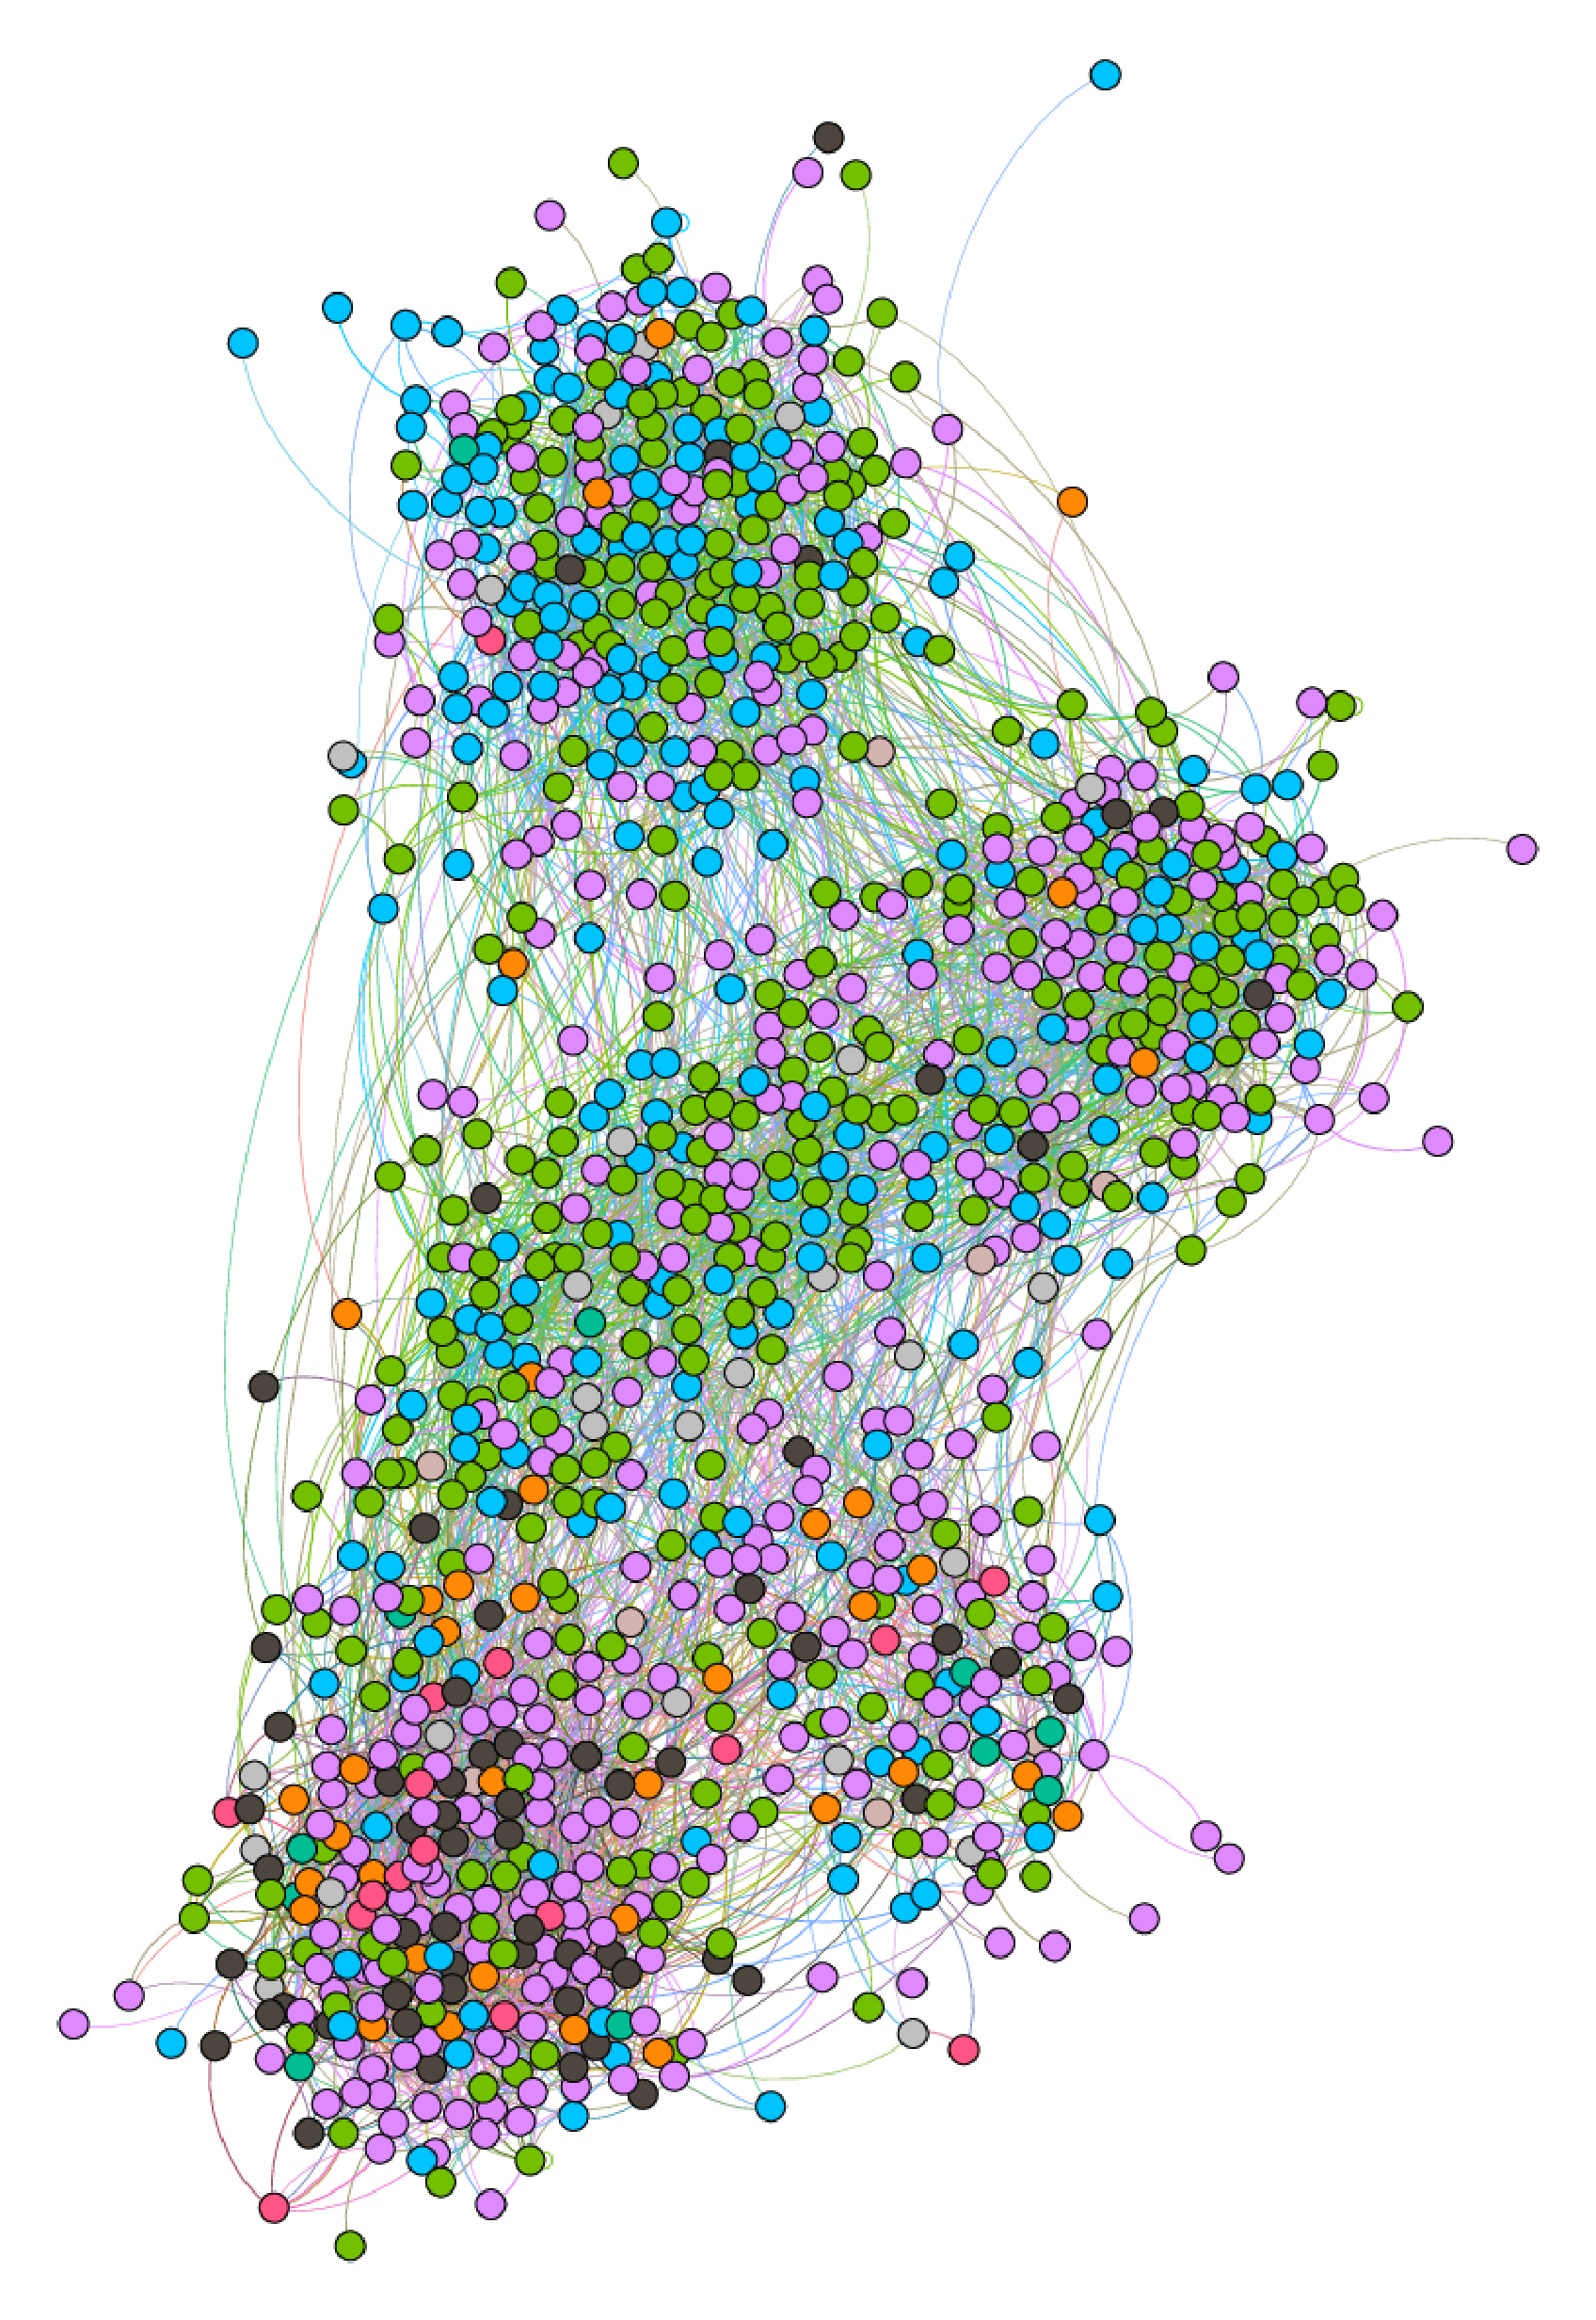
\includegraphics[width=\textwidth]{img/dim5_news.pdf}
    \caption{State vector dimension: 5.
      Latest news highlighted.}
    \label{fig:bubble5news}
  \end{subfigure}
  ~
  \begin{subfigure}[t]{0.35\textwidth}
    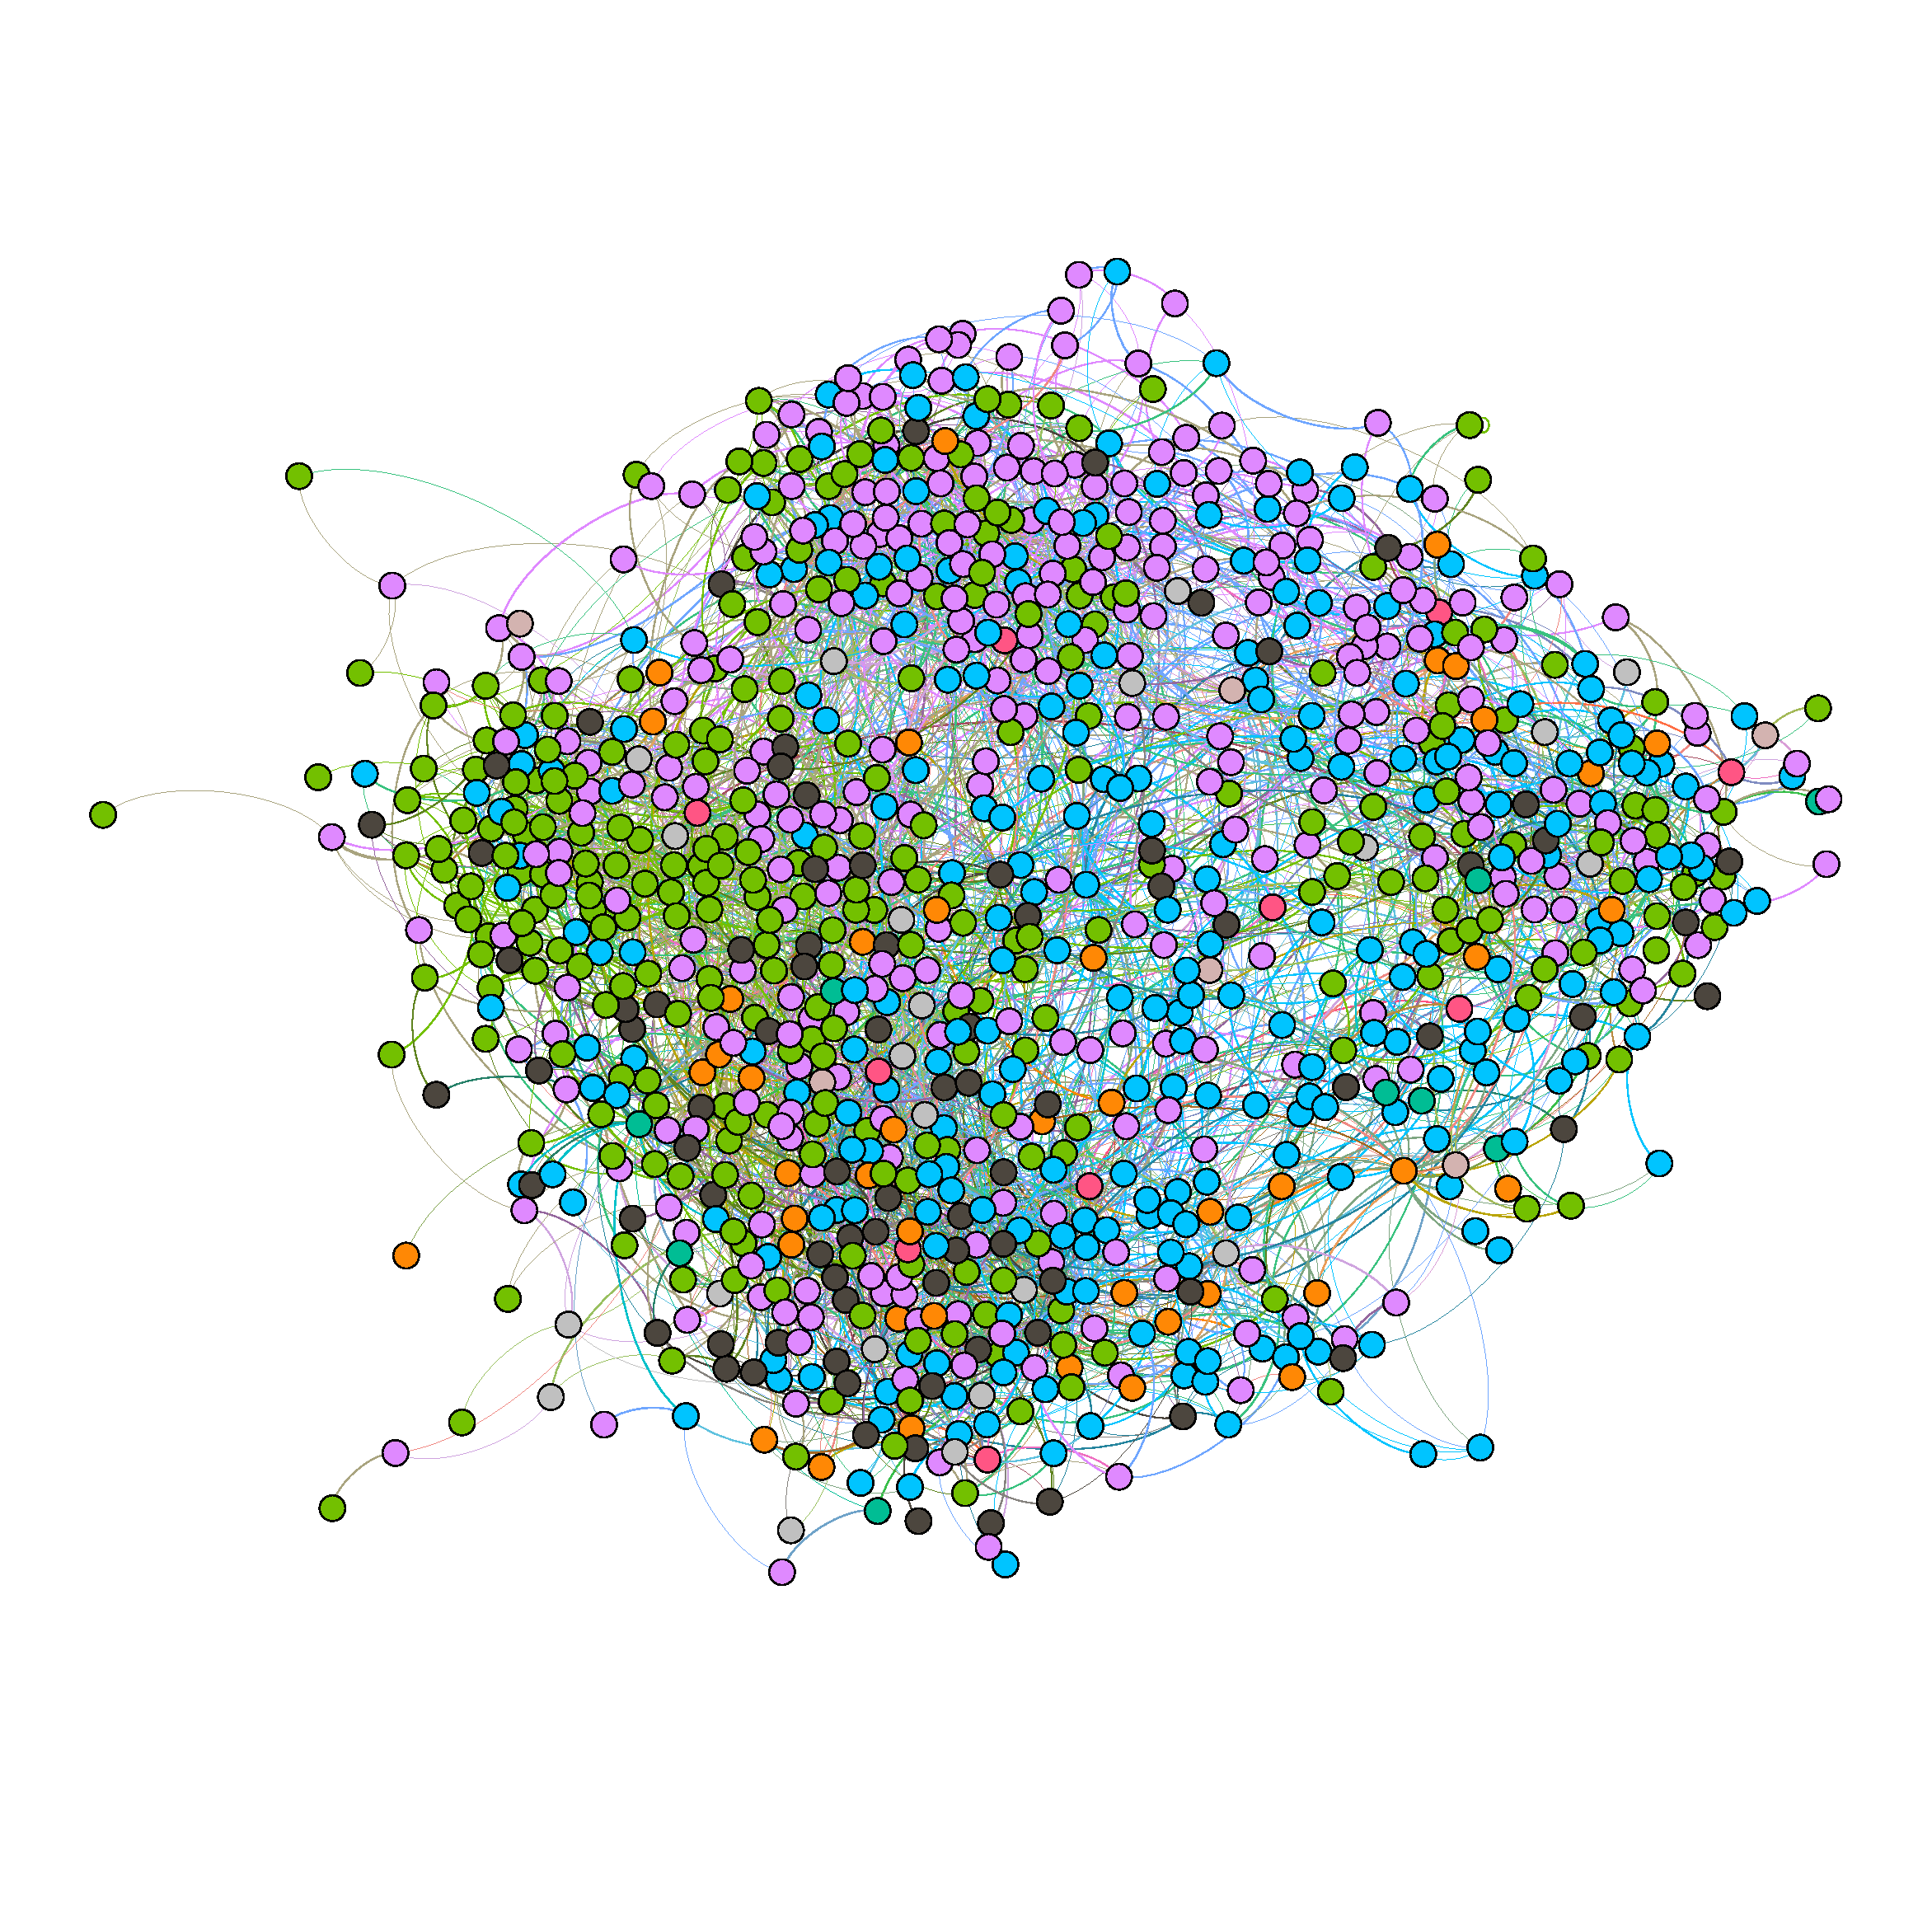
\includegraphics[width=\textwidth]{img/dim7_news.pdf}
    \caption{State vector dimension: 7.
      Latest news highlighted.}
    \label{fig:bubble7news}
  \end{subfigure}
  \caption[Network results: bubble chambers]{Simulations for 1000 users and 20 sources after 1000
    iterations. (\subref{fig:bubble3mod}), (\subref{fig:bubble5mod}) and
    (\subref{fig:bubble7mod}) highlights different modularity classes.
    The number of clusters equals the state vector dimension.
    (\subref{fig:bubble3news}), (\subref{fig:bubble5news})
    (\subref{fig:bubble7news}) highlitghts latest news.
    Clusters clearly depends on state dimension rather than memory
    size. There is not an evident relation with news' behavior
    during the dynamic.
  }
  \label{fig:test}
\end{figure}
